% Fonctionnalité de sauvegarde~:
%% Problématique~: Sauvegarde, reprise sur pannes...
%% Solutions possibles~:
%% Solution choisie \& raisons~:
%%% Implémentation, problèmes rencontrés (temps...), etc.

\subsection{Réponse technique à la sauvegarde et reprise sur panne}
\begin{frame}
\frametitle{Réponse technique à la sauvegarde et reprise sur panne}
\begin{center}

\includegraphics[scale=0.2]{Images/sauvegarde}
\end{center}
\end{frame}

\begin{frame}
\frametitle{Mission de ME~: Réponse technique à la sauvegarde et reprise sur panne}
\begin{block}{\textbf{La sauvegarde : Problématique}}
\begin{itemize}
\item Pas de perte de données
\item Disponibilité
\item Optimisation des flux
\item Coûts
\end{itemize}
\end{block}
\begin{block}{\textbf{Cluster}}
\begin{itemize}
\item groupe logique de serveurs qui s'exécutent simultanément
\item deux postes (configurés comme des serveurs maître/esclave)
\end{itemize}
\end{block}
\end{frame}

\begin{figure}[htbp]
	\centering
	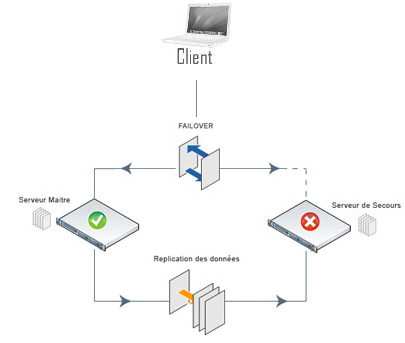
\includegraphics[scale=0.6]{Images/SchemaCluster.png}
	\caption{Cluster, serveur maître et esclave directement connectés}
	\label{SchemaCluster}
\end{figure}

\begin{frame}
\frametitle{}
\begin{block}{\textbf{Fail-Over}}
\begin{itemize}
\item reprise automatique inférieure à une minute
\item mode statique : chaque client est configuré pour basculer sur une URI précise si la standard ne répond plus
\item mode dynamique: le maître fournit dynamiquement l'URI de l'esclave aux clients qui peuvent la mettre à jour
\end{itemize}
\end{block}
\begin{block}{\textbf{Réplication des bases de données en temps réel}}
\begin{itemize}
\item écritures répliquées en temps réel
\item réplication par recopie des journaux de transactions
\item mode synchrone : une transaction émise par un client n'est validée que si l'écriture sur le maître ainsi que la synchronisation avec le serveur de secours sont validées.
\end{itemize}
\end{block}
\end{frame}

\begin{frame}
\begin{block}{\textbf{Procédure de fail-back}}
\begin{itemize}
	\item éteindre le serveur esclave;
	\item copier les données de l'esclave sur le maître;
	\item redémarrer les deux serveurs.
\end{itemize} 
\end{block}
\begin{block}{\textbf{Logiciel}}
\begin{itemize}
	\item Apache Active MQ : agent de messages open source
	\item configurations conservées dans des fichiers XML
\end{itemize} 
\end{block}
\end{frame}
